\documentclass{article}
\usepackage{graphicx}
\graphicspath{{./images/}}
\usepackage[a4paper, margin=2cm]{geometry}
\usepackage[]{enumitem}
\usepackage{float}
\usepackage[]{titling}
\usepackage{hyperref}

\setlength{\droptitle}{-5em}

\title{Assignment 2 Report}
\author{Liam Watson}
\date{\today}

\begin{document}
	
	\maketitle
	
	\section{Introduction}
	This report details answers to key questions posed throughout the Digital Systems Project Assignment and analyses all waveforms given by each module using a Testbench. We aim to highlight key findings and confirm all output behaves as expected after testing.\\
	
	\section{Report 1}
	\begin{figure}[H]
		\centering
		
\includegraphics[width=\linewidth]{q_report1}
		\caption{Screenshot taken from Digital\_Watch\_Part\_2.pdf}
	\end{figure}
	
	In this instance we would prefer to create a new version of this module with a restart feature called \textbf{up\_down\_counter\_rst}. 
	
	\section{Report 2}
	\begin{figure}[H]
		\centering
		
\includegraphics[width=\linewidth]{q_report2}
		\caption{Screenshot taken from Digital\_Watch\_Part\_2.pdf}
	\end{figure}
	
	At this time it appears that verification may not have captured the ability to manually increment up and down nor if we wish to make active changes to \textbf{MAX} or if we wish to change the mininum value for which the counter start. Given our use case these features are not currently intended for our design.
	
	\section{Report 3}
	\begin{figure}[H]
		\centering
		
\includegraphics[width=\linewidth]{q_report3}
		\caption{Screenshot taken from Digital\_Watch\_Part\_2.pdf}
	\end{figure}
	
	When used in a larger design we can use proof by induction which will allow us to say with high confidence that our counter will scale for for higher values of \textbf{MAX}. 
	
	\section{Report 4}
	\begin{figure}[H]
		\centering
		
\includegraphics[width=\linewidth]{q_report4}
		\caption{Screenshot taken from Digital\_Watch\_Part\_2.pdf}
	\end{figure}
	
	\begin{figure}[H]
		\centering
		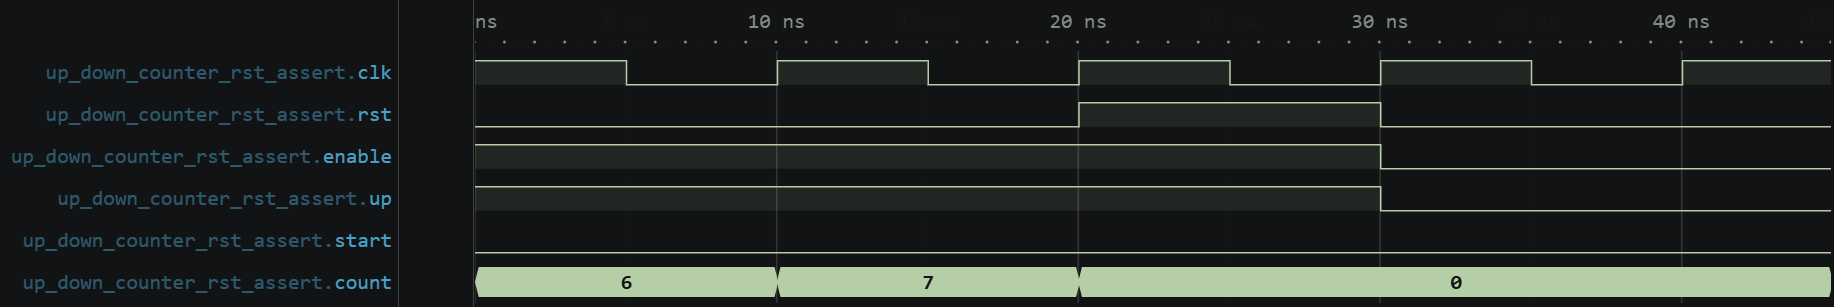
\includegraphics[width=\linewidth]{up_down_counter_rst_assert_waveform}
		\caption{Measured waveform from up\_down\_counter\_rst\_assert}
	\end{figure}
	
	The induction check initialises count to 6. This fails as count then wraps to 0 from a value higher than MAX (4). Restoring the assertion then ensures that MAX can never exceed MAX meaning count can never be set above the value listed in the waveform above.
	
	\section{Report 5}
	
	\begin{figure}[H]
		\centering
		
\includegraphics[width=\linewidth]{q_report5}
		\caption{Screenshot taken from Digital\_Watch\_Part\_2.pdf}
	\end{figure}
	
	\begin{figure}[H]
		\centering
		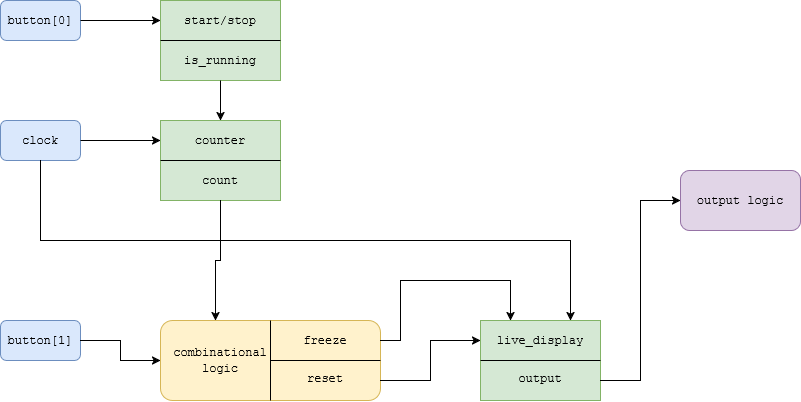
\includegraphics[width=\linewidth]{stopwatch_sketch}
		\caption{Sketch from diagram.io}
	\end{figure}
	
	\section{Report 6}
	
	\begin{figure}[H]
		\centering
		
\includegraphics[width=\linewidth]{q_report6}
		\caption{Screenshot taken from Digital\_Watch\_Part\_2.pdf}
	\end{figure}
	
	I would decompose the stopwatch into several layers. First we would handle our counter module and pass button[0] as an enable to control if the counter is running. I would then create a layer for the live display. I would then use combinational logic to determine the inputs to control the state for live display and use output logic to drive the stopwatch display.  
	
	\section{Report 7}
	
	\begin{figure}[H]
		\centering
		
\includegraphics[width=\linewidth]{q_report7}
		\caption{Screenshot taken from Digital\_Watch\_Part\_2.pdf}
	\end{figure} 
	
	\begin{figure}[H]
		\centering
		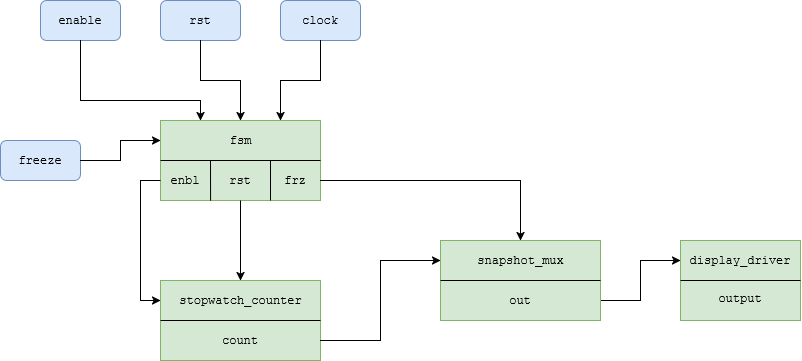
\includegraphics[width=\linewidth]{stopwatch_block_diagram}
		\caption{Block diagram created using diagram.io}
	\end{figure}
	
	
	
\end{document}